\documentclass[11pt,letterpaper]{article}
% Formato comun: sin encabezados ni pies decorativos. Solo numero de pagina.
\usepackage[letterpaper,left=2.3cm,right=2.3cm,top=2.0cm,bottom=2.2cm]{geometry}
\usepackage{fontspec}
\ifdefined\XeTeXgenerateactualtext\XeTeXgenerateactualtext=1\fi
\usepackage[spanish,es-tabla]{babel}
\IfFontExistsTF{Times New Roman}{\setmainfont{Times New Roman}}{\setmainfont{Latin Modern Roman}}
\IfFontExistsTF{Arial}{\setsansfont{Arial}}{\setsansfont{Latin Modern Sans}}
\setmonofont{lmmono10-regular.otf}[Ligatures=NoCommon]
\usepackage{graphicx,longtable,booktabs,array,tabularx,enumitem}
\usepackage{xcolor,hyperref,fvextra,needspace}
\usepackage{xurl}
\hypersetup{hidelinks,pdftitle={FaroNet},pdfauthor={Jimmy Castillo Guzman y Juan Carlos Gomez}}
\urlstyle{same}
\pagestyle{plain}
\setlength{\parindent}{0pt}
\setlength{\parskip}{5pt}
\setlength{\emergencystretch}{2em}
\linespread{1.07}
\setlength{\tabcolsep}{4pt}
\renewcommand{\arraystretch}{1.13}
\setlist[itemize]{nosep,leftmargin=*}
\setlist[enumerate]{nosep,leftmargin=*}
\newcolumntype{P}[1]{>{\raggedright\arraybackslash}p{#1}}
\newcommand{\pendiente}{Pendiente}
\DefineVerbatimEnvironment{codigo}{Verbatim}{fontsize=\small,breaklines=true,breakanywhere=true,breaksymbolleft={},breaksymbolright={},baselinestretch=1.0}
\graphicspath{{figuras/}{../hardware/fotos/}}

\newcommand{\portada}[1]{%
\hypersetup{pageanchor=false}%
\begin{titlepage}
\thispagestyle{empty}
\centering\sffamily\bfseries
\vspace*{0.4cm}
Instituto Tecnológico de Costa Rica\par
\vspace{0.35cm}
Centro Académico de Alajuela\par
\vspace{0.5cm}

\includegraphics[width=4.0cm]{logo-tec.png}\par
\vspace{0.35cm}
CURSO\par
\vspace{0.35cm}
IC-7602: Redes de Computadoras\par
\vspace{0.4cm}
#1\par
\vspace{1.2cm}
Estudiantes:\par
\vspace{0.5cm}
Jimmy Castillo Guzmán\par
\vspace{0.3cm}
Juan Carlos Gómez\par
\vspace{1.2cm}
Profesor:\par
\vspace{0.4cm}
Kevin Moraga\par
\vspace{1.2cm}
Fecha de entrega:\par
\vspace{0.4cm}
1 de noviembre de 2026\par
\vspace{0.7cm}
II Semestre 2026\par
\end{titlepage}
\setcounter{page}{1}
\hypersetup{pageanchor=true}%
}

\begin{document}
\portada{Proyecto 1: FaroNet}

\section{Introducción}

FaroNet integra un enlace construido por el grupo con una red de mensajes
orientada a la privacidad. El problema consiste en transportar datos por luz,
detectar errores, descubrir nodos y encaminar mensajes sin exponer innecesariamente
su contenido ni sus metadatos. La solución combina dos Faros infrarrojos, una
mesh con cifrado por capas y un chat. Un gateway permite publicar en Internet
únicamente los mensajes marcados como públicos.

Cada Faro utiliza una Raspberry Pi 2 conectada por GPIO a su placa. La
comunicación dentro de cada comunidad se realiza sobre UDP en Ethernet o WiFi;
el puente entre comunidades debe realizarse exclusivamente por luz. El diseño
de los protocolos se especifica en el RFC entregado por separado.

\begin{center}
\begin{tabular}{c}
Nodos de comunidad A --- Raspberry + Faro A\\
\textbf{Enlace infrarrojo}\\
Raspberry + Faro B --- Nodos de comunidad B\\[3pt]
Mesh --- Gateway --- HTTPS --- Worker
\end{tabular}
\end{center}

\section{Ambiente de desarrollo}

\begin{tabularx}{\linewidth}{P{3.2cm} X}
\toprule
Área & Herramientas utilizadas\\
\midrule
Hardware & Dos Raspberry Pi 2 Model B de 1 GB, microSD, Raspberry Pi OS de 32 bits y fuentes micro-USB.\\
Montaje & Protoboard MB102, placas perforadas, cautín, estaño, pinzas, alambre y conectores desmontables.\\
Software & Python, pigpio/pigpiod, PyNaCl, gpiozero y pyserial; TypeScript, Node.js y Wrangler para el edge.\\
Pruebas & pytest, Vitest, comprobación de TypeScript y procedimientos de continuidad y tensión con multímetro.\\
Desarrollo & PC, editor de texto, terminal SSH, Git y GitHub.\\
Documentación & LaTeX, RFC ASCII, fotografías y diagramas vectoriales.\\
\bottomrule
\end{tabularx}

El trabajo se organiza por cambios pequeños en Git: implementar, ejecutar las
pruebas correspondientes, revisar el diff y publicar el commit. Las llaves y
contraseñas se mantienen fuera del repositorio. Para depurar se comprueban por
separado niveles del detector, bytes recibidos, tramas con CRC y mensajes de red.

Repositorio del grupo:
\url{https://github.com/JuankGO/redes-proyecto1-faronet}.

\section{Diseño}

\subsection{Faro y conexiones}

El emisor es un LED IR limitado por 330~ohmios y controlado por un transistor
NPN 2N2222A. GPIO17 llega a su base por 2,2~kiloohmios y una resistencia de
10~kiloohmios une base y GND. El PT333 conecta su emisor a GND y su colector a
RX, con un pull-up de 10~kiloohmios hacia 3,3~V. Dos LEDs indican TX/RX, un
condensador de 100~nF desacopla la alimentación y el botón conecta GPIO24 a GND.

Con luz RX vale 0 y sin luz vale 1. El programa invierte la recepción UART.
La electrónica externa se alimenta a 3,3~V; la Raspberry conserva su alimentación
normal por micro-USB. La variante de emisor a 5~V no se considera implementada.
Se usan headers para retirar la Raspberry sin desoldar. Las patas B/C/E se
identifican por la referencia del transistor, no únicamente por su apariencia.

\begin{center}
\begin{minipage}[t]{0.49\linewidth}
\vspace{0pt}\small
\begin{tabular}{lrr}
\toprule
Señal & GPIO BCM & Pin físico\\
\midrule
3,3 V & -- & 1\\
GND & -- & 6\\
TX & 17 & 11\\
RX & 27 & 13\\
Indicador TX & 22 & 15\\
Indicador RX & 23 & 16\\
Botón de pánico & 24 & 18\\
\bottomrule
\end{tabular}
\end{minipage}\hfill
\begin{minipage}[t]{0.47\linewidth}
\vspace{0pt}\small\raggedright
La figura siguiente muestra las piezas y conexiones en una distribución de
referencia sobre placa perforada. Los trazos finos representan pistas inferiores
y los gruesos, cables aislados. El esquema eléctrico complementario se conserva
en \path{docs/hardware/esquematico-faro.svg}.
\end{minipage}
\end{center}

\begin{figure}[!htbp]
\centering
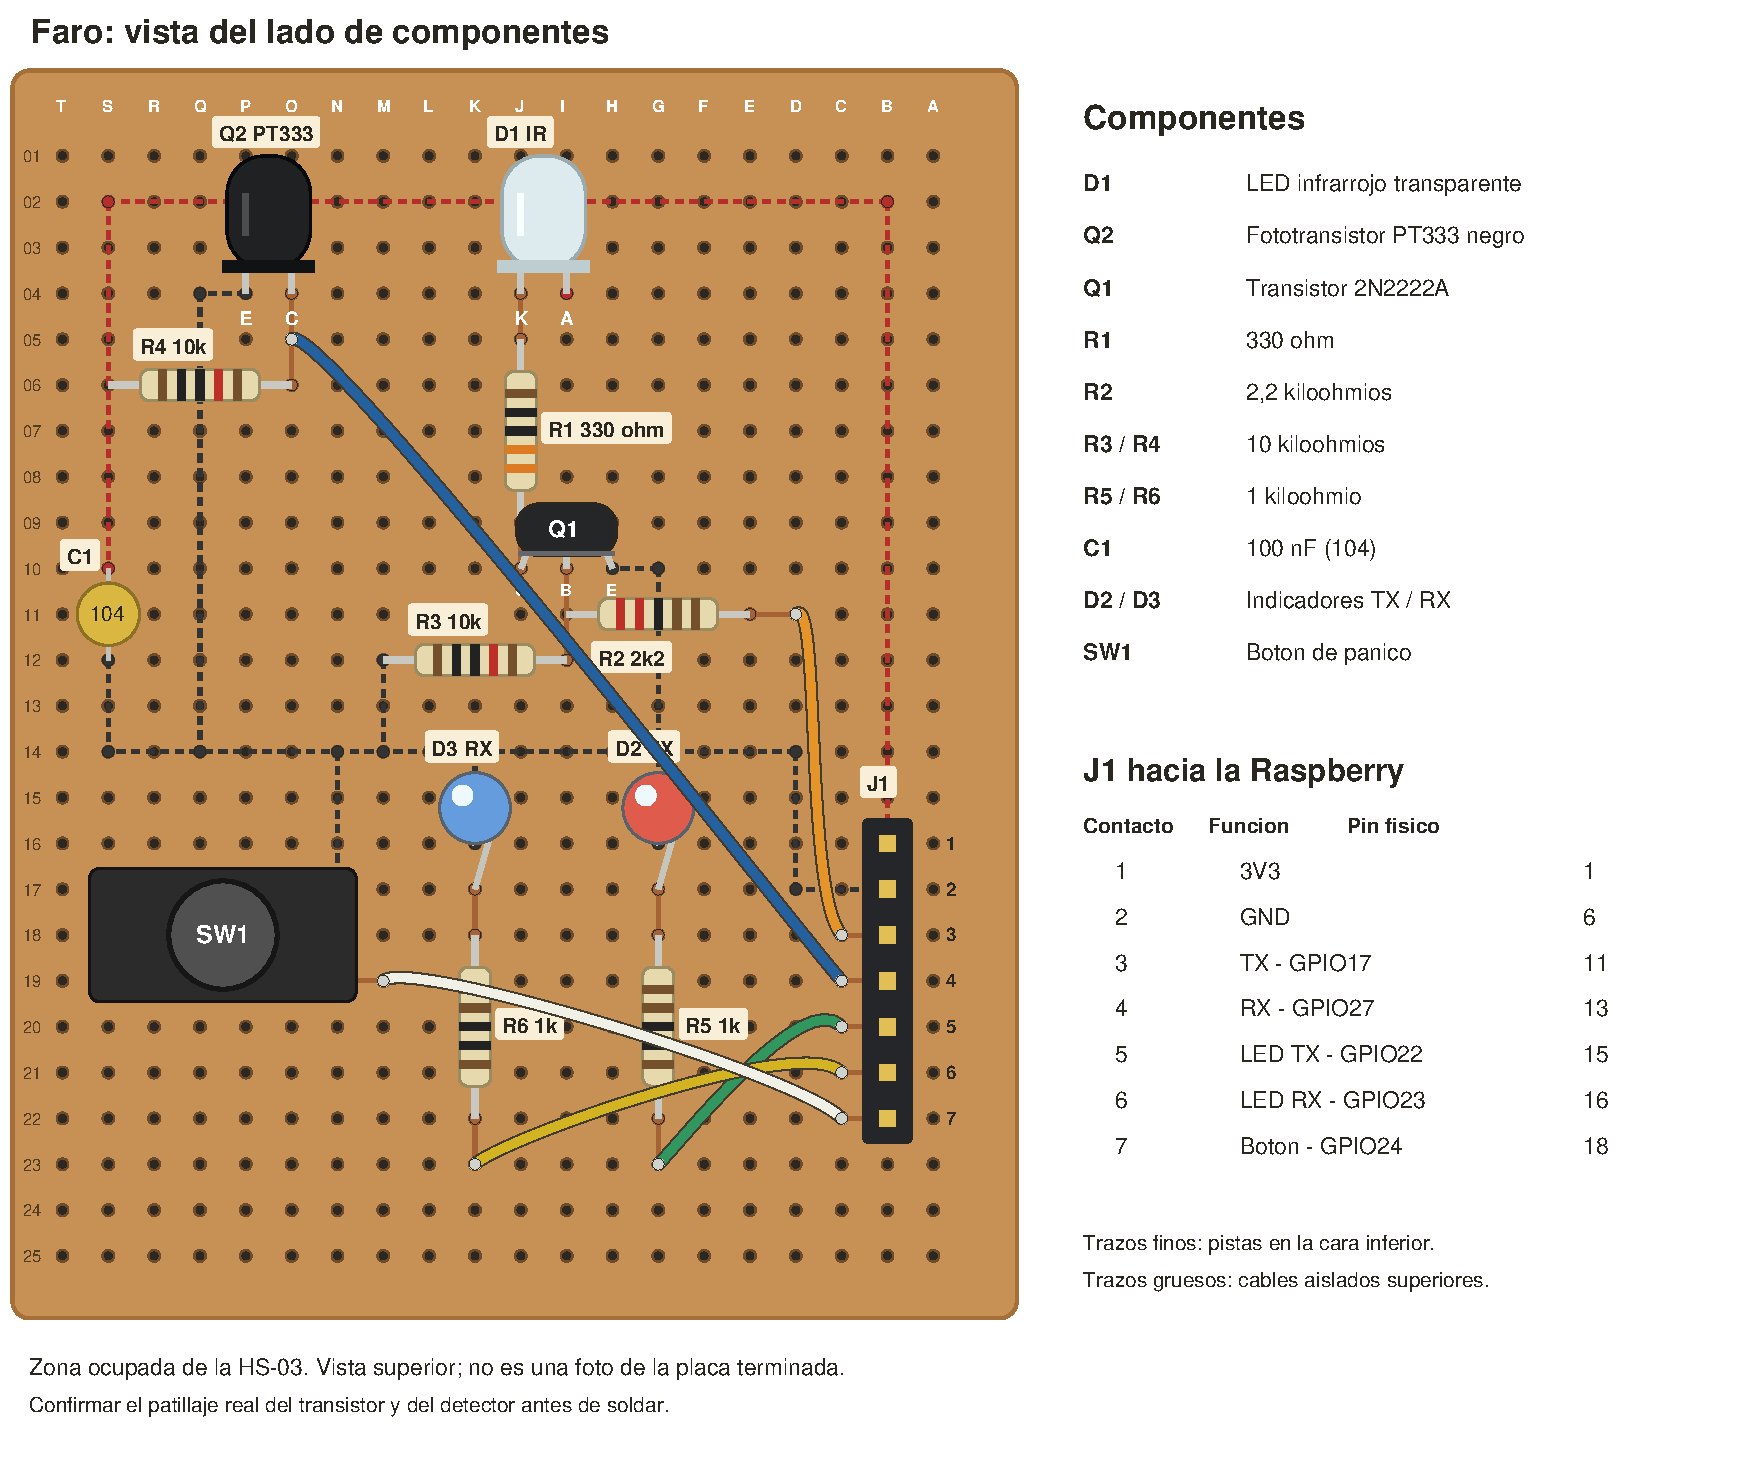
\includegraphics[width=\linewidth]{montaje-faro.pdf}
\caption{Vista de montaje del Faro por el lado de componentes.}
\end{figure}

\clearpage
\subsection{Lista de materiales}

Las cantidades corresponden a los dos Faros. Los costos son estimaciones en
colones para valorar las piezas del kit, no comprobantes de compra. No incluyen
el valor de las Raspberry, microSD y herramientas que ya estaban disponibles.

{\small
\begin{longtable}{P{8.5cm} r r r}
\toprule
Material & Cantidad & CRC / unidad & Subtotal CRC\\
\midrule\endhead
D1: LED IR compatible con PT333, nominalmente 940 nm & 2 & 350 & 700\\
Q2: Fototransistor PT333 negro & 2 & 900 & 1800\\
Q1: NPN 2N2222A & 2 & 447 & 894\\
R1: Resistencia 330 ohmios, 1/4 W & 2 & 50 & 100\\
R2: Resistencia 2,2 kiloohmios, 1/4 W & 2 & 50 & 100\\
R3, R4: Resistencia 10 kiloohmios, 1/4 W & 4 & 50 & 200\\
R5, R6: Resistencia 1 kiloohmio, 1/4 W & 4 & 50 & 200\\
C1: Cerámico 100 nF, código 104 & 2 & 100 & 200\\
D2, D3: LED visible TX y RX, colores disponibles & 4 & 100 & 400\\
SW1: Pulsador normalmente abierto & 2 & 250 & 500\\
J1: Tira de header de siete contactos, paso 2,54 mm & 2 & 200 & 400\\
Cableado: Cables desmontables compatibles con los headers & 14 & 50 & 700\\
Placa: Perforada de islas, HS-03 o equivalente & 2 & 1000 & 2000\\
Puentes: Porción de alambre aislado por placa & 2 & 200 & 400\\
Consumible: Porción de estaño y flux por placa & 2 & 250 & 500\\
TOTAL & - & - & 9094\\
\bottomrule
\end{longtable}}


Las fuentes, cables de red, PC y protoboard son recursos adicionales reutilizados.
El multímetro es necesario para registrar continuidad, ausencia de cortos y
voltajes. El consumo del LED se verifica midiendo su resistencia limitadora;
un cálculo teórico no se presenta como corriente medida.

\subsection{Fotografías y pruebas eléctricas}

Se dispone de una fotografía del prototipo y de la cara de componentes de una
placa soldada. Faltan las vistas finales de ambas caras del Faro A y la cara de
cobre del Faro B. La protoboard documenta el desarrollo y no sustituye el Faro
soldado requerido para la revisión.

\begin{figure}[!htbp]
\centering
\begin{minipage}{0.46\linewidth}
\centering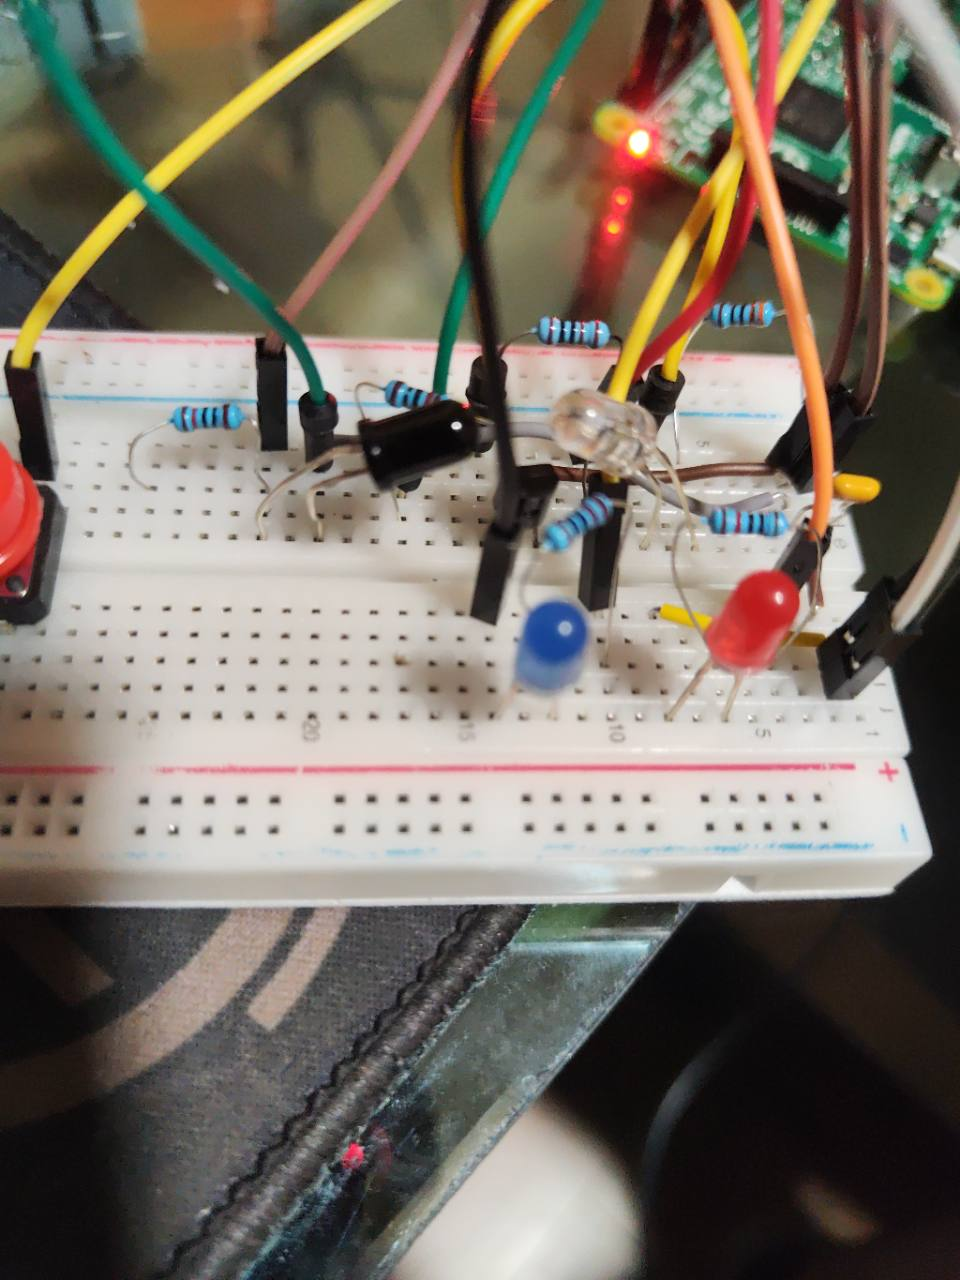
\includegraphics[height=5.0cm,keepaspectratio]{prototipo-a.jpg}
\par\small Prototipo en MB102.
\end{minipage}\hfill
\begin{minipage}{0.46\linewidth}
\centering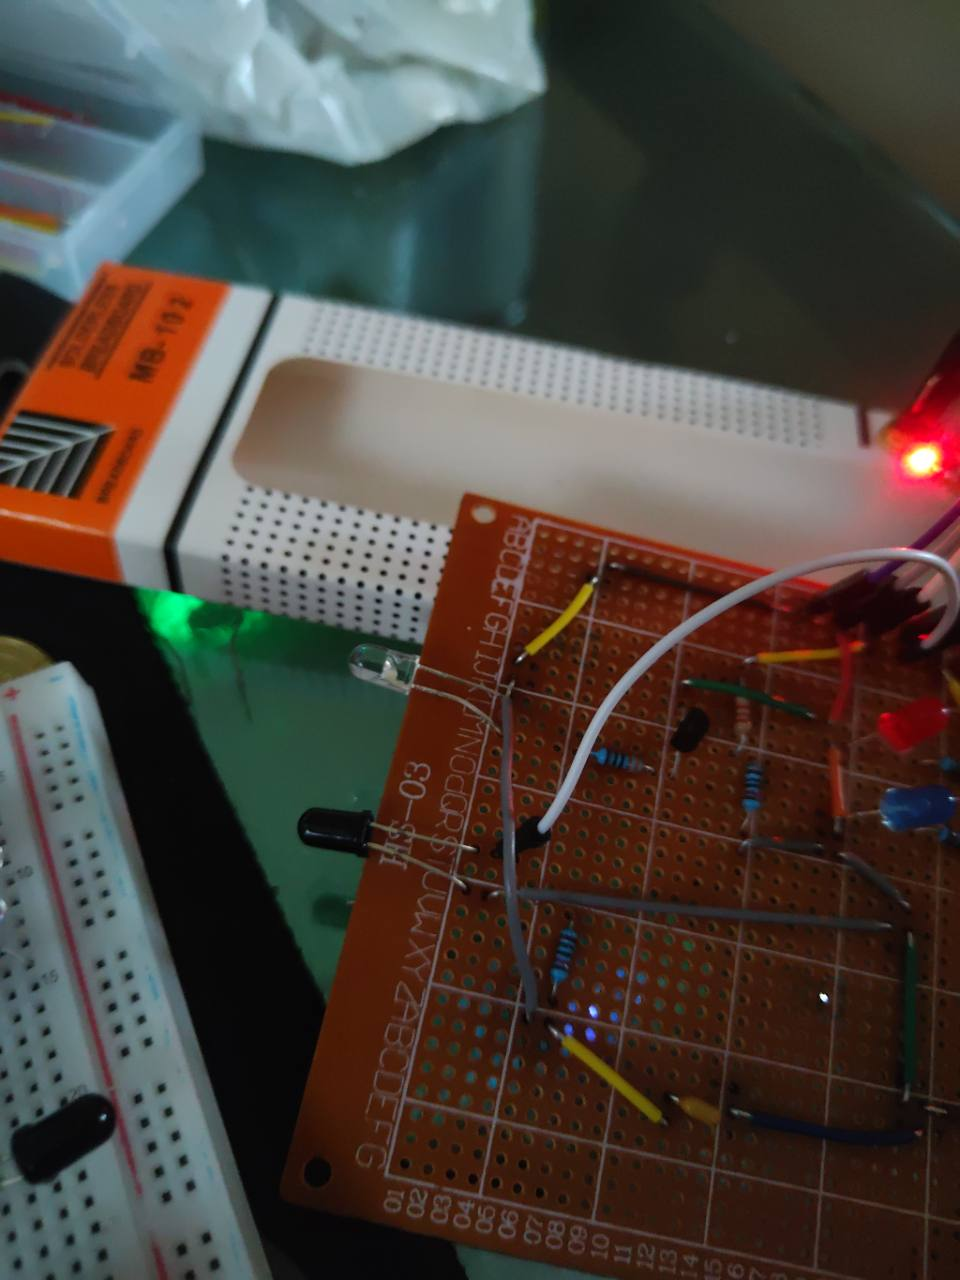
\includegraphics[height=5.0cm,keepaspectratio]{faro-b-componentes.jpg}
\par\small Placa soldada, componentes.
\end{minipage}
\caption{Evidencia fotográfica disponible del desarrollo.}
\end{figure}

No se recibieron medidas de multímetro. La tabla conserva los valores pendientes;
las lecturas digitales de GPIO no sustituyen la medición. Continuidad y cortos se
comprueban sin energía; para tensión se toma GND como referencia.

{\small
\begin{longtable}{P{6.3cm} P{4.1cm} P{1.4cm} P{1.4cm}}
\toprule
Comprobación & Condición esperada & Faro A & Faro B\\
\midrule\endhead
Continuidad de 3V3, GND y señales hasta J1 & Cada segmento llega a su destino & \pendiente & \pendiente\\
Ausencia de corto entre VCC y GND & Sin puente directo estable & \pendiente & \pendiente\\
Resistencias y patillaje de semiconductores & Coinciden con el esquema & \pendiente & \pendiente\\
Alimentación de la placa & Cercana a 3,3 V & \pendiente & \pendiente\\
Base de Q1 con TX activo & Unión B-E conduciendo & \pendiente & \pendiente\\
Colector de Q1 con TX activo & Nivel bajo & \pendiente & \pendiente\\
RX con detector oscuro & Cercano a 3,3 V & \pendiente & \pendiente\\
RX con luz enfrentada & Nivel bajo, objetivo menor a 0,5 V & \pendiente & \pendiente\\
Caída en 330 ohmios & Registrar para calcular I=V/330 & \pendiente & \pendiente\\
Botón suelto / presionado & Alto con pull-up / bajo & \pendiente & \pendiente\\
\bottomrule
\end{longtable}}

\subsection{Protocolo físico}

La trama tiene 12 bytes de cabecera, hasta 114 de contenido y 2 de CRC; su máximo
es 128 bytes. Declara versión, tipo, origen, destino, secuencia y longitud.
CRC-16/CCITT-FALSE detecta errores accidentales. Manchester se aplica al
preámbulo, delimitador y trama; los medios bits se empaquetan en UART 8N1.
Una trama máxima usa 266 bytes UART más un auxiliar de pigpio, sin cambiar el
límite de la trama lógica.

El adaptador espera silencio del canal y usa retroceso aleatorio. DATA dirigida
espera ACK y admite reintentos; la difusión no confirma recepción. Las direcciones
físicas son de cuatro bytes y se guardan en microSD. El nodo las rota al arrancar,
periódicamente y al activar pánico. La biblioteca acepta tramas externas válidas.

Se inicia explícitamente a 300 baudios y se ajusta solo después de medir el enlace.
La tasa útil y BER deben medirse a tres distancias con luz ambiental normal.
Se proponen 1, 2 y 5 cm; los resultados están pendientes y no se sustituyen por
la velocidad configurada ni por una prueba simulada.

{\small
\begin{tabularx}{\linewidth}{l l X X X}
\toprule
Distancia & Sentido & Recibidas / enviadas & BER & Tasa útil B/s\\
\midrule
1 cm & A a B / B a A & Pendiente & Pendiente & Pendiente\\
2 cm & A a B / B a A & Pendiente & Pendiente & Pendiente\\
5 cm & A a B / B a A & Pendiente & Pendiente & Pendiente\\
\bottomrule
\end{tabularx}}

La herramienta de BER compara contenidos conocidos y cuenta todos los bits de
una trama perdida como erróneos. La tasa útil divide el payload confirmado entre
el tiempo total, incluyendo ACK y reintentos. Hay que registrar fecha, luz,
distancia, baudios, cantidad de tramas y resistencia del receptor en cada sesión.

\subsection{Mesh, aplicación y edge}

La mesh usa UDP y Faro. HELLO descubre vecinos; un directorio intercambia entradas
firmadas, y las rutas se actualizan por costo en saltos y vencimiento. Los mensajes
de aplicación miden 256 bytes y las celdas 1024 bytes con relleno aleatorio.
PyNaCl construye una cebolla de tres relays. La selección exige cinco candidatos
además de origen y destino, por lo que la demostración anónima necesita siete nodos.
Los mensajes se fragmentan en el enlace óptico y se reensamblan al otro lado.

El chat distingue mensajes privados, temas privados con frase compartida y
mensajes públicos. Solo los públicos salen por el gateway. Las peticiones al
Worker se autentican con Ed25519, marca de tiempo y nonce. El Worker implementa
salas con Durable Objects y WebSockets, feeds Atom, directorio firmado, límite
de peticiones y buzón de blobs cifrados de 1024 bytes, con TTL y borrado al leer.
El despliegue tiene configuración Wrangler y migraciones D1 versionadas.

URL informada por el grupo:
\url{https://faronet-worker.faronet-jimmy-juan.workers.dev}.
El Worker se implementó, pero no se utilizó en la demostración integrada.

\subsection{Modelo de amenazas y decisiones de privacidad}

{\small
\begin{tabularx}{\linewidth}{P{2.8cm} X X}
\toprule
Adversario & Información observable & Defensa y límite\\
\midrule
Nodo malicioso & Vecino anterior, siguiente salto y tiempos & Cebolla y padding; persiste correlación por colusión.\\
Observador óptico & Actividad, duración y cabeceras físicas & Cifrado superior y direcciones rotables; la demo cruda no es privada.\\
Operador del gateway & Públicos y conexión al Worker & Filtra privados; ve los datos que se publican.\\
Proveedor del edge & IP de conexión, tiempos y contenido público & La aplicación no registra encabezados, pero el proveedor observa su infraestructura.\\
Acceso al dispositivo & Llaves y estado en sistema o microSD & Pánico y borrado lógico; no garantizan borrado forense en flash.\\
\bottomrule
\end{tabularx}}

No se implementan primitivas criptográficas propias. Los mensajes y entradas
tienen TTL; no se escriben bitácoras persistentes de usuarios. El directorio sí
publica direcciones operativas para enrutar y, por tanto, expone metadatos.
No se promete anonimato ante un observador global, Sybil o un sistema operativo
comprometido. HELLO y RUTA no están firmados en v1. El botón de GPIO24 borra
estado sensible de forma lógica, renueva identidad y activa los indicadores.

\section{Estructuras de datos usadas y funciones}

Los enteros binarios de varios bytes usan orden de red. El formato y los campos
están definidos en el RFC; la siguiente tabla identifica las estructuras y las
funciones principales del código.

{\small
\begin{longtable}{P{3.5cm} P{4.1cm} P{5.5cm}}
\toprule
Módulo & Estructura o función & Responsabilidad\\
\midrule\endhead
\texttt{faro.frame} & \texttt{Trama}, \texttt{codificar}, \texttt{decodificar}, \texttt{crc16} & Validar cabecera, longitudes, versión y CRC; construir bytes de trama.\\
\texttt{faro.linea} & \texttt{armar\_senal}, \texttt{extraer\_trama} & Manchester, preámbulo, delimitador y recuperación de trama.\\
\texttt{faro.serie\_pigpio} & \texttt{SeriePigpio}, buffer de bytes & UART por GPIO17/27, inversión RX, envío por ondas y cierre del lector.\\
\texttt{DispositivoLuz\allowbreak{}Adaptador} & Secuencia, pendientes y contadores & Acceso al medio, ACK, reintentos y duplicados; \texttt{enviar\_crudo} valida tramas externas.\\
Identidad y pánico & Llaves, dirección y archivos locales & Crear, persistir, rotar y borrar estado; \texttt{Nodo.panico} renueva identidad y vacía tablas.\\
Vecinos y rutas & \texttt{TablaVecinos}, \texttt{TablaRutas} & Registrar vecinos directos, costos y vencimientos.\\
Directorio & \texttt{Directorio}, \texttt{firmar}, \texttt{verificar} & Comprobar estructura, vigencia y firma de entradas.\\
Celda y cebolla & \texttt{empaquetar\_celda}, \texttt{construir\_cebolla} & Relleno a 1024 bytes y cifrado con PyNaCl para destino y relays.\\
Enlace Faro & Cola y tabla de fragmentos & Partir mensajes en datos de hasta 110 bytes más índice/total; reensamblar y vencer parciales.\\
Aplicación & Mensaje fijo y \texttt{Cliente} & Empaquetar 256 bytes, validar TTL y manejar privado, tema y público.\\
Gateway & Cola y encabezados firmados & Filtrar privados y publicar mensajes públicos mediante HTTPS autenticado.\\
Worker & \texttt{Sala}, HTTP y cron & Salas, WebSocket, Atom, buzón, directorio y limpieza de vencidos.\\
\bottomrule
\end{longtable}}

La biblioteca expone \texttt{enviar}, \texttt{enviar\_confiable},
\texttt{enviar\_crudo}, \texttt{recibir} y \texttt{cambiar\_direccion}.
Una sola hebra utiliza la instancia. Los módulos mantienen docstrings y
comentarios; las pruebas verifican límites, errores y formatos sin sustituir
las comprobaciones físicas.

\section{Instrucciones para ejecutar el programa}

\subsection{Preparación y comprobación}

Grabar Raspberry Pi OS Lite de 32 bits con Raspberry Pi Imager, configurar
usuario y red y conectar la placa siguiendo el mapa GPIO. El Faro ejecuta Python
en Linux: no necesita compilar ni flashear otro firmware. En cada Raspberry:

\begin{codigo}
sudo apt update
sudo apt install -y git pigpiod python3-pigpio python3-nacl \
  python3-serial python3-gpiozero python3-pytest
sudo systemctl enable --now pigpiod
git clone https://github.com/JuankGO/redes-proyecto1-faronet.git faronet-juank
cd faronet-juank
python3 -m pytest tests -q
python3 -m faro.medir loopback --uart pigpio --baudios 300 --tramas 5
\end{codigo}

Si ya existe una copia con cambios locales, conservarla y usar otra carpeta para
la nueva copia. El loopback requiere que el LED mire al detector de la misma
placa. Un solo proceso debe controlar los GPIO de cada Raspberry. No se activa
la UART de hardware de los GPIO14/15 para este montaje.

Para comprobar texto, primero en B y después en A, desde la raíz del repositorio:

\begin{codigo}
# B recibe
python3 -u -m faro.demo_recibir --uart pigpio --baudios 300
# A envia
python3 -u -m faro.demo_enviar --uart pigpio --baudios 300 \
  --destino ffffffff --mensaje "Hola Faro B"
\end{codigo}

La difusión no espera confirmación: el texto debe aparecer en B. Para ACK,
sustituir \texttt{ffffffff} por la dirección física hexadecimal que imprime B.
Estas demos de diagnóstico no incorporan el cifrado del chat.

\subsection{Tasa útil y BER}

Para BER, ejecutar el receptor B antes del emisor A. Repetir con las distancias
reales y después invertir los papeles:

\begin{codigo}
# B, ejemplo a 1 cm
python3 -m faro.medir recibir --uart pigpio --baudios 300 \
  --tramas 100 --espera 120 --distancia 0.01
# A
python3 -m faro.medir enviar --uart pigpio --baudios 300 \
  --tramas 100 --pausa 1
\end{codigo}

La pausa supera el silencio de veinte tiempos de byte que delimita las ráfagas.
Para tasa con ACK, ejecutar primero el eco y luego el emisor:

\begin{codigo}
# B
python3 -m faro.medir eco --uart pigpio --baudios 300
# A
python3 -m faro.medir tasa --uart pigpio --baudios 300 \
  --tramas 20 --espera-ack 10 --distancia 0.01
\end{codigo}

Registrar resultados a 1, 2 y 5 cm, bajo luz ambiental normal. Cien tramas máximas
a 300 baudios requieren aproximadamente 17 minutos con pausas; no realizar toda
la medición durante la defensa.

\subsection{Nodos y chat}

La operación anónima exige siete participantes: dos chats con Faro, cuatro relays
y un gateway. Se pueden usar procesos distintos en una PC con puertos y carpetas
separadas. Sustituir IP de ejemplo por las reales. La comunidad B no debe tener
una ruta UDP alternativa hacia A para demostrar el puente exclusivo por luz.

En A, con IP de ejemplo 192.168.10.10 y una PC semilla 192.168.10.20:

\begin{codigo}
python3 -m app.chat --nodo 192.168.10.10:7001 --alias jimmy \
  --uart pigpio --baudios 300 --semilla 192.168.10.20:7101 \
  --carpeta ~/.faronet-a
\end{codigo}

En B, por ejemplo 192.168.20.10, sin semilla IP hacia A:

\begin{codigo}
python3 -m app.chat --nodo 192.168.20.10:7002 --alias juan \
  --uart pigpio --baudios 300 --carpeta ~/.faronet-b
\end{codigo}

Cuatro relays en terminales separadas de la PC:

\begin{codigo}
python3 -m mesh.nodo --puerto 7101 --ip-publica 192.168.10.20 \
  --semilla 192.168.10.10:7001 --carpeta ~/.faronet-r1
python3 -m mesh.nodo --puerto 7102 --ip-publica 192.168.10.20 \
  --semilla 192.168.10.10:7001 --carpeta ~/.faronet-r2
python3 -m mesh.nodo --puerto 7103 --ip-publica 192.168.10.20 \
  --semilla 192.168.10.10:7001 --carpeta ~/.faronet-r3
python3 -m mesh.nodo --puerto 7104 --ip-publica 192.168.10.20 \
  --semilla 192.168.10.10:7001 --carpeta ~/.faronet-r4
\end{codigo}

El séptimo proceso es el gateway de la siguiente sección. Esperar a que el
directorio reúna cinco candidatos útiles además de los dos extremos. En el chat:

\begin{codigo}
/nodos
/priv PREFIJO_ID_DESTINO Hola por FaroNet
/unirse equipo frase-compartida-larga
/tema equipo Mensaje del tema privado
/publico noticias Mensaje publico
/panico
/salir
\end{codigo}

Usar el prefijo que muestre \texttt{/nodos}. El modo \texttt{--permitir-directo}
sirve solo para pruebas y no acredita los tres relays. El botón de GPIO24 hace el
borrado mientras corre el nodo, chat o gateway con el Faro activado.

\subsection{Despliegue reproducible del Worker}

El Worker no se utilizó en la demostración integrada. Estos pasos documentan
cómo reproducir el código existente, con cuenta Cloudflare y plan gratuito.
Desde \texttt{worker}:

\begin{codigo}
npm ci
npx tsc --noEmit
npx vitest run
npx wrangler login
\end{codigo}

Para una cuenta nueva, crear la base y colocar su identificador en
\texttt{wrangler.jsonc} antes de aplicar las migraciones:

\begin{codigo}
npx wrangler d1 create faronet-db
npx wrangler d1 migrations apply faronet-db --remote
\end{codigo}

Crear la identidad del gateway desde la raíz del repositorio y copiar solo su
llave pública, nunca el archivo privado:

\begin{codigo}
python3 -c "from pathlib import Path; \
from faro.identidad import cargar_o_crear; \
f,_=cargar_o_crear(Path.home()/'.faronet-gw'); \
print(f.verify_key.encode().hex())"
\end{codigo}

Desde \texttt{worker}, guardar esa llave y desplegar:

\begin{codigo}
npx wrangler secret put GATEWAY_PUB
npx wrangler deploy
\end{codigo}

La URL real se toma de Wrangler. El ejemplo utiliza la informada por el grupo.
El gateway usa la misma carpeta con la que se creó la llave:

\begin{codigo}
python3 -m gateway.gateway --puerto 7200 --ip-publica 192.168.10.20 \
  --semilla 192.168.10.10:7001 --carpeta ~/.faronet-gw \
  --worker https://faronet-worker.faronet-jimmy-juan.workers.dev
\end{codigo}

Las rutas públicas son \texttt{/sala/noticias}, \texttt{/feed/noticias.atom}
y \texttt{/directorio}. Para desarrollo local se usa \texttt{npx wrangler dev}
con \texttt{.dev.vars}, que no se sube al repositorio. Desde la raíz,
\texttt{python3 tools/prueba\_buzon.py http://localhost:8787} comprueba depósito,
lectura, eliminación y tamaño del buzón.

\section{Actividades realizadas por estudiante}

El grupo estimó unas veinte horas-persona durante tres fines de semana. La tabla
es una reconstrucción aproximada: se reparten diez horas por integrante, no un
registro cronometrado. Las fechas se interpretan como 17--18 y 24--25 de octubre,
y 31 de octubre--1 de noviembre de 2026. Algunas actividades incluyen revisión
y pruebas de código escrito antes de esas fechas.

\Needspace{18\baselineskip}
\subsection*{Jimmy Castillo Guzmán}
{\small
\begin{longtable}{P{2.1cm} P{10.8cm} r}
\toprule
Fecha estimada & Actividad & Horas\\
\midrule\endhead
2026-10-17 & Revisar materiales, resistencias y funciones del emisor y detector & 1,5\\
2026-10-18 & Montar prototipo y revisar GPIO, indicadores y botón & 1,5\\
2026-10-24 & Preparar distribución y soldar componentes de una placa & 2,0\\
2026-10-25 & Revisar uniones, jumpers y alineación óptica del prototipo & 1,0\\
2026-10-31 & Completar montaje soldado y adaptar el puerto a GPIO17/27 & 2,0\\
2026-11-01 & Configurar Raspberry, probar por SSH y revisar evidencias y documentación & 2,0\\
TOTAL & Jimmy & 10,0\\
\bottomrule
\end{longtable}}

\Needspace{18\baselineskip}
\subsection*{Juan Carlos Gómez}
{\small
\begin{longtable}{P{2.1cm} P{10.8cm} r}
\toprule
Fecha estimada & Actividad & Horas\\
\midrule\endhead
2026-10-17 & Revisar tramas, CRC y pruebas de la biblioteca del Faro & 2,0\\
2026-10-18 & Revisar directorio firmado, rutas y simulaciones de la mesh & 2,0\\
2026-10-24 & Ajustar y probar cifrado por capas y comandos del chat & 2,0\\
2026-10-25 & Revisar código y configuración del Worker, gateway y pruebas locales & 2,0\\
2026-10-31 & Apoyar revisión de integración, materiales y casos de prueba & 1,0\\
2026-11-01 & Revisar RFC, resultados y documentación de entrega & 1,0\\
TOTAL & Juan Carlos & 10,0\\
\bottomrule
\end{longtable}}


\textbf{Total Jimmy: 10 horas. Total Juan: 10 horas. Total del grupo: 20 horas-persona.}

\section{Autoevaluación}

\subsection{Estado, problemas y limitaciones}

Se aprobaron 140 pruebas Python, 23 del Worker local y la comprobación de
TypeScript. Esto valida partes del software, no soldaduras, voltajes ni alcance.
El grupo reportó un loopback de protoboard estable a 1000 baudios; no reemplaza
las mediciones formales de tasa útil y BER a tres distancias.

El diagnóstico entre los dos Faros no confirmó recepción válida: ambas Raspberry
generaban pulsos TX, pero no se recuperó una secuencia útil en el otro extremo.
Se requiere comprobar el acondicionamiento de RX y el camino óptico. Las
mediciones de multímetro y las fotografías finales faltantes permanecen pendientes.
El Worker se implementó y se probó localmente, pero no se utilizó integrado.

Persisten límites de correlación de tráfico, anuncios HELLO/RUTA sin firma,
exposición de direcciones en el directorio y borrado no forense en microSD.
La pista que muestra el chat no autentica por sí sola al emisor de un privado.
La fragmentación y los anuncios son lentos a 300 baudios; el puente físico
completo no se presenta como una prueba aprobada.

\subsection{Rúbrica del proyecto}

Las notas son una propuesta de autoevaluación basada en la evidencia disponible,
para revisión por ambos integrantes. No son calificaciones del profesor.

{\small
\begin{tabularx}{\linewidth}{X r r}
\toprule
Rubro & Peso & Nota propuesta / 10\\
\midrule
Hardware soldado, esquema, BOM y pruebas & 25\% & 4\\
Capa 1 y DispositivoLuzAdaptador & 10\% & 6\\
Capas 2 y 3: mesh y directorio & 15\% & 8\\
Privacidad & 10\% & 7\\
Aplicación anónima & 5\% & 8\\
Aplicación pública en el edge & 25\% & 6\\
RFC & 5\% & 9\\
Documentación & 5\% & 8\\
\midrule
Resultado ponderado propuesto & 100\% & 62,5 / 100\\
\bottomrule
\end{tabularx}}

El hardware tiene evidencia parcial y requiere validación; la capa física no ha
demostrado el enlace entre placas. Mesh y aplicación cuentan con pruebas de
software. El edge se implementó sin utilizarse en la integración. RFC y
documentación incluyen lo exigido, con evidencia pendiente expresamente indicada.

\subsection{Aprendizaje}

Escala: 1 muy malo, 2 malo, 3 regular, 4 bueno y 5 muy bueno. Las siguientes
valoraciones son propuestas que cada integrante debe revisar.

{\small
\begin{tabularx}{\linewidth}{X r r}
\toprule
Rubro & Jimmy & Juan\\
\midrule
Soldadura y hardware & 4 & 3\\
Capa física & 4 & 4\\
Enrutamiento mesh & 3 & 4\\
Privacidad y anonimato & 4 & 4\\
Serverless en el edge & 3 & 4\\
Redacción de RFC & 4 & 4\\
\bottomrule
\end{tabularx}}

\subsection{Reporte de commits}

El historial conserva autor, fecha y descripción; no se usa para deducir horas.
Los alias de Git se agrupan bajo Jimmy y Juan para facilitar su lectura. El
corte del reporte es anterior al commit de esta revisión documental.

{\footnotesize
\begin{longtable}{P{1.3cm} P{1.8cm} P{1.2cm} P{9.3cm}}
\toprule
Commit & Fecha & Autor & Descripción\\
\midrule\endhead
c4234a3 & 2026-11-01 & Jimmy & Conservar PDF y fotografias como archivos binarios\\
4da62e1 & 2026-11-01 & Jimmy & Documentar entrega FaroNet y unificar montaje GPIO17/27\\
891e5eb & 2026-10-30 & Jimmy & test(faro): scripts de prueba cruda de emisor y receptor por UART\\
c7a3b9b & 2026-10-30 & Juan & Merge pull request \#4 from JuankGO/faro-simplificado\\
f4538c1 & 2026-10-30 & Jimmy & feat(faro): modo loopback en faro.medir para probar un solo Faro\\
77cf357 & 2026-10-30 & Juan & Merge pull request \#3 from JuankGO/main\\
8a30954 & 2026-10-30 & Juan & Merge pull request \#2 from JuankGO/faro-simplificado\\
ba70abd & 2026-10-30 & Jimmy & docs(faro): documentar el Faro simplificado sin comparador\\
1c7e8a9 & 2026-10-26 & Jimmy & Merge pull request \#1 from JuankGO/ACACHETE\\
f054099 & 2026-10-26 & Jimmy & build(Nuevo): Juank no sabe nada, yo si\\
f9e5990 & 2026-10-17 & Juan & Worker de Cloudflare desplegado con D1 y Durable Objects\\
ffdf247 & 2026-10-16 & Juan & Integración Mesh + Chat completada\\
ce04044 & 2026-10-15 & Juan & Prueba de integracion de la mesh\\
8ecfa5c & 2026-10-14 & Juan & Directorio firmado con TTL y tabla de vecinos\\
972d72a & 2026-10-12 & Juan & Parte 7 completa: identidad, panico y cebolla\\
55c0558 & 2026-10-12 & Juan & Parte 7A: identidad criptografica del nodo (Ed25519 + Curve25519)\\
386170c & 2026-10-12 & Juan & Modelo de amenazas v1\\
064cd70 & 2026-10-12 & Juan & Demo del medio simulado entre dos Faros\\
fe44373 & 2026-10-12 & Juan & Capa 1: trama Faro v1 con CRC, Manchester y DispositivoLuzAdaptador\\
10139f8 & 2026-10-12 & Juan & Estructura inicial del repositorio\\
b77a1c2 & 2026-09-30 & Juan & Initial commit\\
\bottomrule
\end{longtable}}


\section{Lecciones aprendidas}

\begin{itemize}
\item Comprobar niveles del detector antes de buscar errores de trama o de rutas.
\item Mantener el mismo mapa GPIO y la misma polaridad en código y diagrama.
\item Distinguir transmisión de recepción: la difusión no garantiza entrega.
\item Medir continuidad sin alimentación y registrar voltajes antes de conectar GPIO.
\item Aislar el receptor del LED propio y reservar margen de velocidad y alineación.
\item Separar pruebas de códec, transporte, cifrado, aplicación y despliegue.
\item Registrar horas y evidencias durante el trabajo, no únicamente al final.
\item Describir límites de anonimato y borrado sin prometer seguridad absoluta.
\end{itemize}

\section{Bibliografía}

\begin{enumerate}[label={[\arabic*]}]
\item Moraga, K. \emph{Proyecto 1: FaroNet}. Redes de Computadoras, TEC, septiembre de 2026.
\item RFC Editor. RFC 7322, \emph{RFC Style Guide}. \url{https://www.rfc-editor.org/rfc/rfc7322}
\item RFC Editor. RFC 6973, \emph{Privacy Considerations for Internet Protocols}. \url{https://www.rfc-editor.org/rfc/rfc6973}
\item PyNaCl. Documentación de la biblioteca. \url{https://pynacl.readthedocs.io/en/latest/}
\item pigpio. Interfaz Python. \url{https://abyz.me.uk/rpi/pigpio/python.html}
\item Raspberry Pi. Documentación de GPIO. \url{https://www.raspberrypi.com/documentation/computers/raspberry-pi.html}
\item Cloudflare. Wrangler y D1. \url{https://developers.cloudflare.com/workers/wrangler/commands/} y \url{https://developers.cloudflare.com/d1/wrangler-commands/}
\item Código e historial de FaroNet. \url{https://github.com/JuankGO/redes-proyecto1-faronet}
\end{enumerate}

\end{document}
